\documentclass[journal]{article}

\usepackage{amsmath}
\usepackage{graphicx}
\usepackage[english]{babel}
\usepackage[a4paper,margin=1in,footskip=0.25in]{geometry}

\usepackage{mathtools}
\DeclarePairedDelimiter\bra{\langle}{\rvert}
\DeclarePairedDelimiter\ket{\lvert}{\rangle}
\DeclarePairedDelimiterX\braket[2]{\langle}{\rangle}{#1 \delimsize\vert #2}

\begin{document}
\title{Qurry: A prototype quantum programming language}

\author{Lucas~Saldyt}

\markboth{Journal}
{Journal}

\maketitle

\begin{abstract}
     The core philosophy of Qurry is that simple language features, in aggregate, can make quantum programming significantly easier, by offering lightweight abstractions in the spirit of modern C++.
    This allows users to implement quantum algorithms cleanly, without glossing over necessary lower-level details of quantum computing, such as the abstract topology of a particular computer.
    Qurry takes a top-down approach, moving from the abstract goal of creating higher-order functions and datatypes to the level of individual language features.
    While the desired semantics of a true quantum programming language are not yet completely crystalized, the creation of simple language abstractions will elevate the level at which quantum programs are thought about, potentially enlightening the creation of a true quantum programming language.
    Many existing quantum programming languages are truly circuit languages, with few features above the level of gates, and sometimes rudimentary functions or macros, and there is currently a tendency not to stray very far from this model.
    Lastly, Qurry is not just a language, but a software ecosystem which is meant to catalyze the development of quantum programming languages.
\end{abstract}

\section{Introduction}

Innovation in near-term quantum programming requires the use of lightweight abstractions, which allow users to easily exploit the power of quantum computing while still understanding its fundamental mechanisms \cite{stroustrup}.
In 1981, Richard Feynman noted that quantum physics appears to be impossible to simulate using a classical computer, but that quantum computers appeared to be perfectly capable of simulating quantum physics \cite{feynman_1981}.
Effectively, quantum computation potentially allows new problems to be computed efficiently: in particular, this includes literal simulations of the physical world, but also abstract algorithms which may receive a superpolynomial change in time complexity.
Qurry allows quantum programmers to access the power of quantum computers, without sacrificing performance or understanding of the underlying mechanisms.

\subsection{Motivation}

Stephen Jordan, of Microsoft, keeps a nearly exhaustive list of quantum algorithms and the speedups that they offer \cite{jordan}.
According to this list at time of writing, there are thirty-five distinct quantum algorithms which offer a potential superpolynomial speedup.
This famously includes Peter Shor's factoring and discrete log algorithms, as well as, fundamentally, quantum simulation.
Interestingly, many quantum algorithms such as the Deutsch-Jozsa algorithm are matched (at least practically, and sometimes theoretically) by probabilistic algorithms, and even some algorithms with superpolynomial speedups are based on older probabilistic versions.
For instance, machine learning does not appear to have superpolynomial improvements at time of writing.
The most promising application of quantum computing in the near term is in molecular simulation.
As the comparisons section will demonstrate, Qurry offers unique programming language features which implementing each of these algorithms significantly easier.

% At time of writing, quantum computers have been used to simulate di-Hydrogen, Be-H2, and [Other small molecules, Cite]
% [Qurry aims to assist in the development and implementation of each of these algorithms...]
% 
% Quantum computing [motivations]
% [TODO: General motivations, cite Rigetti, cite Haskell/LISP/Rich Hickey, cite Probabilistic programming languages]
% [Cite Peter Selinger's papers]

\subsection{Background}

The absolute basics of quantum computing are not nearly as intimidating as they are sometimes made out to be.
The main requirement is linear algebra, but complex numbers and probability are also helpful. 
Conventionally, quantum data is represented on qubits.
When measured, qubits will be in *either* of two states: $\ket{0}$ or $\ket{1}$.
However, more generally, qubits are in a combination of these two states, which is known as a superposition.
A particular active qubit's state is described by two complex numbers, $\alpha$ and $\beta$, which are collected in a vector.
This is written in the simple equation: $$\ket{\psi} = \alpha\ket{0} + \beta\ket{1}$$.
However, the state vector $\alpha, \beta$ is not directly examinable.
Instead, when a qubit is measured, one measures $\ket{0}$ with probability $|\alpha|^2$, and $1$ with probability $|\beta|^2$, which must sum to $\ket{1}$.
For single qubits, a state is evolved in the model simply by multiplying the state vector for a qubit by a $2$ by $2$ unitary matrix, known as a one-qubit gate. This is written as $Av$.

For $n$ qubits, the state is simply a complex vector of length $2^n$, and a $n$ qubit gate is a $2^n \text{ by } 2^n$ matrix:
$$\ket{\psi} = \alpha_i\ket{s_i} \text{ for } s_i \in \{\{0, 1\}^n\}, 0 < i < 2^n - 1$$.
Once a given $n$-qubit quantum state is measured, the outcome is a single bit-string, $s_i$, with probability $|\alpha_i|^2$.
If it is possible to repeat this measurement (by preparing the quantum state multiple times), then a collection of measurements is a multinomial distribution defined by the states $s_i$ and probabilities $\alpha_i$, but this distribution has $2^n$ states, and measuring a quantum state only gives a single sample.

Importantly, past a single qubit, quantum states can be entangled.
Two states are entangled when the measurement outcome of one qubit is correlated with the measurement outcome of other qubits.
The simplest, most famous example of this is the Bell states, also known as EPR pairs.
For instance, in one Bell state, two qubits are either measured both as $\ket{0}$, or both as $\ket{1}$ (even when measured independently), but there is no probability for them to differ.
This is the basis for all interesting quantum algorithms.

To summarize, superposition is the fundamental state model for quantum computers, but a given quantum state cannot be measured directly, only sampled once.
Then, entanglement allows the correlation of measurements, which is a crucial ingredient in any useful quantum algorithm. 
Any quantum program is simply a combination of linear operators which affect the superposition.
Given an initial state, conventionally the zero vector, a quantum program $P$ operates on the state vector, and then the vector is sampled, by measuring a subset of its qubits.
Importantly, a quantum program $P$ is itself a linear operator, potentially further composed of other linear operators.
The data in a quantum program, at this level of abstraction, will only ever be a vector of qubits, but at higher levels of abstraction, this vector can be subsectioned into semantic datatypes, no differently than how C++'s fundamental memory model is a sequence of bytes.

At the same time, in hybrid classical-quantum computation, classical control can setup, run, and measure the outcomes of quantum sub-programs.
In this way, some quantum program $P$ will be embedded in a hybrid program.

\subsection{Circuit Languages}

At time of writing, Rigetti pyquil contains the following quantum gates and operations:

Single qubit gates and operations:

\begin{itemize}
    \item RESET, I, X, Y, Z, H, S, T
\end{itemize}

Qubit gates taking an angle as the the parameter and qubit as the second:

\begin{itemize}
    \item RX, RY, RZ, PHASE
\end{itemize}

Swap operators, where each takes two qubits, and PSWAP takes an additional angle as a first argument:

\begin{itemize}
    \item SWAP, ISWAP, and PSWAP
\end{itemize}

Controlled operators:

\begin{itemize}
    \item CZ, CNOT %['control', 'target']
    \item CSWAP %['control', 'target\_1', 'target\_2']
    \item CPHASE00, CPHASE01, CPHASE10, CPHASE %['angle', 'control', 'target']
\end{itemize}

And of course the hybrid measurement instruction, which takes a qubit as the first argument, and a classical register as the second:

\begin{itemize}
    \item MEASURE
\end{itemize}

And also contains the following classical operations:

\begin{itemize}
    \item TRUE, FALSE, NOT, NEG %['classical\_reg']
    \item AND, OR, MOVE, EXCHANGE, IOR, XOR %['classical\_reg1', 'classical\_reg2']
    \item ADD, SUB, MUL, DIV %['classical\_reg', 'right']
    \item EQ, GT, GE, LE, LT %['classical\_reg1', 'classical\_reg2', 'classical\_reg3']
    \item LOAD %['target\_reg', 'region\_name', 'offset\_reg']
    \item STORE %['region\_name', 'offset\_reg', 'source']
    \item CONVERT %['classical\_reg1', 'classical\_reg2']
\end{itemize}

Most importantly, though, QUIL actually already has a notion of higher-level functions, which it calls ``Modifiers".
These are the following:
\begin{itemize}
    \item DAGGER
    \item CONTROLLED
\end{itemize}

\subsection{Classical Probabilistic Languages}

 Classical probabilistic programming languages are a recent innovation from the MIT cognitive science community. 
 Essentially, they create a way for non-expert programmers to access the power of Bayesian inference. 
 Users can create simple probabilistic models in standard code, and then run them through an expert-created inference backend.
 Famously, this has resulted in dramatically reduced code complexity, with a famous case where a 50-line probabilistic program could compete with traditional approaches to face recognition [TODO: Cite].

 Qurry is inspired by the effects these languages have had, and in fact there is some overlap between quantum programming and classical probabilistic languages.
 For instance, quantum bayesian inference has been conceptualized since the 70s-90s [Cite].
 There are 10-billion cool libraries that use quantum bayesian inference [Cite].

\subsection{Parallels to C++ and its role in the classical software ecosystem}

Lightweight abstractions, as defined by Bjarne Stroustrup, are abstractions that lower the cognitive load on the user, without sacrificing understanding of the underlying processes behind particular code \cite{stroustrup}.

In Bjarne's words:
``The aim [of C++] is to allow a programmer to work at the highest feasible level of abstraction by providing a simple and direct mapping to hardware and zero-overhead abstraction mechanisms"

Layers of abstraction are a fundamental idea in all of computer science, and quantum computing is no different.
Currently, quantum computing operates on the abstraction that is the gate-level, where programs are defined by gates acting sequentially on particular qubits, and users conventionally do not need to be aware about every hardware detail of their quantum computer.
The universal gate model of quantum computing generally allows a quantum programmer to ignore many details of the quantum computer they are running on: Sources of error aside, a quantum program on an ion-trap computer should behave in the same way as the same program on a computer which uses superconducting qubits, in much the same way that a conventional C++ program does not need to worry about the CPU architecture of the computer it is running on, because (generally), these details are
handled by the compiler.
It is precisely abstractions like these which make programming possible in the first place.

However, some have argued for the importance of hardware, as in Google's phrase ``hardware aware, not hardware agnostic". [TODO: Cite]
Many aspects of hardware are particularly important, for instance, topology, which will potentially result in a programmer needing to modify a quantum algorithm for it to run on two separate computers.
Additionally, the error generation of a quantum computer is actually a crucial detail, even though quantum programmers might desire to ignore it.
In the current state of quantum computing, many details of hardware cannot yet be ignored. 
However, it is obvious that \emph{eventual} hardware independence is desirable --- Consider the power of Java in the classical computing world. Lightweight abstractions are precisely the scaffold that will catalyze this transition.

\section{Features}

    Creating abstractions in quantum programming languages comes down to the creation of higher-order functions and higher-order datatypes.
    Language features that allow the creation and composition of both higher-order functions and higher-order datatypes set Qurry apart from lower-level circuit languages.

    \subsection{Higher Order Functions}

    The simplest illustration of a higher order function is trivial, but surprisingly neglected from any existing quantum language: it is the tensor operator ($U^{\otimes n}$), known to functional programmers as the higher-order function, \emph{map}.
    Many quantum algorithms will begin with a change of basis, effectively a state preparation. 
    Commonly, this is to the Hadamard basis, and is done by applying the Hadamard operator to a block of qubits.
    In a conventional circuit language, this is done as the following:
    \begin{verbatim}
    H 0
    H 1
    ...
    H n\end{verbatim}
    However, textbooks and papers will write this as $H^{\otimes n}$, and in Qurry, it can be written:
    \begin{verbatim}
    (define workspace (block n qubit))
    (map H workspace)\end{verbatim}
    Implicitly, this example also introduces Qurry's assignment statement \emph{define}, and its representation for qubit arrays, the $block$ command, which takes a size and a type, and allocates space and handles mapping to actual qubit indices.
    More impressively, Qurry supports automatic currying of functions:
    \begin{verbatim}
    (define initialize_basis (map H))
    (define workspace (block n qubit))
    (initialize_basis workspace)\end{verbatim}

    Of course, Qurry utilizes the two existing higher-order functions defined by QUIL: DAGGER, and more importantly, CONTROLLED.
    For brevity, Qurry redefines CONTROLLED to CU.
    Effectively, this allows the creation of arbitrary controlled operators, for instance the redefinition of CNOT:
    \begin{verbatim}
    (define custom_cnot (CU X))
    (H 0)
    (custom_cnot 0 1)
    \end{verbatim}
    Qurry calls functions like CU controlled higher level operators.
    This list includes:
    \begin{itemize}
        \item CU 
        \item CNU
        \item Cascade, CascadeU
        \item ReverseCascade, ReverseCascadeU
        \item Collect, CollectU
        \item Expand, ExpandU
        \item SimU
    \end{itemize}
    Interestingly, many of these are defined through composition of simpler gates.
    For instance, CNU takes a block of control qubits and a block of work qubits, and entangles pairs of control and work qubits, and finally entangles a target qubit, which a unitary is controlled by:
    [TODO: Circuit Diagram]
    A ``Cascade" is simply a chain of shifted CNOT gates, and a ``CascadeU" is simply a ``Cascade" which in turn controls the operation of a unitary gate.
    [Circuit Diagram]
    ReverseCascade:
    [Circuit Diagram]
    Now consider the circuit used for the simulation of a hamiltonian:
    [Circuit Diagram]
    Clearly, this circuit contains repeated information, which can be abstracted into the form of another function: ``SimU", which in turn is a "collect" operation, an "expand" operation, and a controlled unitary in between them.
    [Circuit Diagram]

    \subsection{Higher Order Datatypes}

    Qurry's memory model is simple: an array of $n$ qubits, and $m$ classical bits.
    However, in programmer-space, these arrays are cut up and defined using semantic datatypes.

    The previous section discussed the \emph{block} type, and the \emph{define} command.
    The \emph{block} command will automatically select appropriate qubits in the array, and map to these when used.

    In terms of datatypes, not much more is needed, except for the \emph{datatype} command, which mimics C++'s \emph{struct} or \emph{class}.
    For simplicity, elegance, and robustness, Qurry does not implement encapsulation or inheritance, but instead uses public access by default (in the spirit of Python, since after all, Qurry has a Python interface), and relies on composition instead of inheritance.
    A \emph{datatype} is nothing more than a contiguous collection of other Qurry datatypes, with names for each field.
    Like \emph{block} objects, \emph{datatype}s automatically map to qubits and bits in Qurry's memory model.
    These can be \emph{block}s, single qubits, single bits, and other defined \emph{datatype} objects, allowing for recursive types.
    Fields within a datatype are simply accessed with the dot operator:
    % TODO: should functions be possible as datatype fields?
    \begin{verbatim}
        (datatype entanglion
                  (a qubit)
                  (b qubit))
        (define e (entanglion))
        (H e.a)
        (CNOT e.a e.b)
    \end{verbatim}

    Recursively composed higher-order datatypes, in combination with recursively composed higher-order functions are the foundation for creating a more abstract programming language.

    \subsection{Other Features}

    \begin{itemize}
        \item clear 	    
        \item cond 	    
        \item do 	        
        \item macro 	    
    \end{itemize}


 \section{Comparisons}
    This section is currently commented out.
% 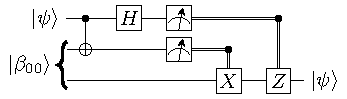
\includegraphics{teleport.pdf}
% 
%     Draw examples from Nielsen and Chuang, and the general literature.
% 
%  Simply change (if (condition) (branch) (branch))
%  into
%  ``
%  Condition
%  Measure []
%  Jump label
%  branch
%  branch etc
%  ``
%  
%  Curry also supports variable naming, blocks of qubits, classical callbacks, imports, \dots
%  Curry can be called as a library and operated from python
%  
%  There are some easy targets for providing abstraction: common things like functions, conditionals, loops, integer data types, and so on. 
%  However, let's jump into the quantum/probabilistic side of things.
%  
%  Models will fundamentally be composed of, generally, wave functions: Superpositions over all possible states.
%  First, consider modeling a classical distribution. 
%  We can successfully produce sampleable classical distributions on a quantum computer.
%  For instance, consider the following model from the Church programming language tutorial.
%  This code is specifying a probabilistic grammar for simple sentences about cooking.
%  
%  ```scheme
%  (define (transition nonterminal)
%    (case nonterminal
%          (('D) (multinomial(list (list (terminal 'the))
%                                  (list (terminal 'a)))
%                            (list (/ 1 2) (/ 1 2))))
%          (('N) (multinomial (list (list (terminal 'chef))
%                                   (list (terminal 'soup))
%                                   (list (terminal 'omelet)))
%                             (list (/ 1 3) (/ 1 3) (/ 1 3))))
%          (('V) (multinomial (list (list (terminal 'cooks))
%                                   (list (terminal 'works)))
%                             (list (/ 1 2) (/ 1 2))))
%          (('A) (multinomial (list (list (terminal 'diligently)))
%                             (list (/ 1 1))))
%          (('AP) (multinomial (list (list 'A))
%                              (list (/ 1 1))))
%          (('NP) (multinomial (list (list 'D 'N))
%                              (list (/ 1 1))))
%          (('VP) (multinomial (list (list 'V 'AP)
%                                    (list 'V 'NP))
%                              (list (/ 1 2) (/ 1 2))))
%          (('S) (multinomial (list (list 'NP 'VP))
%                             (list (/ 1 1))))
%          (else 'error)))
%  ```
%  
%  More succinctly, this is specifying the following (toy) language model:
%  ```scheme
%  D(eterminer):      (uniform 'the' 'a')
%  N(oun):            (uniform 'chef' 'omelet' 'soup')
%  V(erb):            (uniform 'cooks' 'works')
%  A(dverb):          (uniform 'diligently')
%  AP(Adverb Phrase): (uniform A)
%  NP(Noun Phrase):   (D, N)
%  VP(Verb Phrase):   (uniform (V AP) (V NP))
%  S(entence):        (NP, VP)
%  ```
%  
%  To make things even simpler, let's first just consider modeling a randomly sampled Noun-Phrase (which is the first part in sampling a full toy sentence).
%  The noun-phrase is a concatenation of a determiner and a noun. In our toy example, we have two determiners and three nouns, both uniformly sampled, which makes for a total of six options with equal probability.
%  So, we'll need three qubits to model this. Curry has builtins for these distributions.
%  ```scheme
%  (def determiner-qubit 0)
%  (def noun-qubits 1 2)
%  (bernoulli 0.5 determiner-qubit)
%  (multinomial 0.33 0.33 0.34 noun-qubits)
%  ```
%  
%  The output is the following (using a local simulator):
%  ```
%  grid {curry}: ./compile examples/test.lisp
%  
%  [['def', 'determiner-qubit', '0'],
%   ['def', 'noun-qubits', '1', '2'],
%   ['bernoulli', '0.5', 'determiner-qubit'],
%   ['multinomial', '0.33', '0.33', '0.34', 'noun-qubits']]
%  
%  {'000': 0.17, '001': 0.16, '010': 0.17, '011': 0.17, '100': 0.16, '101': 0.16}
%  
%  277.4035930633545 ms simulated runtime
%  ```
%  
%  In our output, the rightmost bit is representing the determiner, and the other two bits are representing the noun.
%  So the output is:
%  ```python3
%  {'the chef' : 1/6, 'a chef' : 1/6, 'the omelet' : 1/6, 'a omelet' : 1/6, 'the soup' : 1/6, 'a soup' : 1/6}
%  ```
%  Now, let's consider the rest of the model.
%  When we sample a Verb Phrase, it contains recursive elements.
%  So, it will branch (with equal probabilities) to either (V AP) or (V NP).
%  Before diving in, let's look at branching in quantum computers.
%  
%  Consider preparing a bell state:
%  ```
%  (h 0)
%  (cnot 0 1)
%  ```
%  And distinguish this from the following, which will produce the same classical measurements, but no entanglement (because the state of the first qubit is known before producing the state in the second qubit). 
%  In this case, the state 01 is possible, because the first qubit may be measured in the 1 state, and the second qubit is unprepared, and in the zero state.
%  ```
%  (bernoulli 0.5 0)
%  (measure 0 0)
%  (if 0 (x 1) (nop))
%  ```
%  
%  So, when creating a probabilistic model which branches, we distinguish between these two types of branching, because only one truly creates an entangled state.
%  However, this makes representing information slightly more difficult, because we will not know which bits correspond to which states (unless we encode this, which we will).

\section{Software Ecosystem}

In addition to being a prototype quantum programming language, Qurry defines a software stack surrounding the language, which is intended to make development more pleasant.
For instance, this software stack makes it exceptionally easy to add new language features and libraries to Qurry.
This allows one to rapidly test new ideas in quantum programming and let the language evolve on its own as opposed to architecting a top-down ``perfect'' language.

\section{Standard Library}

    Qurry contains mechanisms which enable easy inclusion of qurry code in the form of libraries.
    As an example, Qurry's standard library is implemented in this fashion.

    Explain how the statistics library can be easily implemented.

    At time of writing, Qurry contains the following constructs:  	
    \begin{itemize}
	    \item gaussian 	
        \item bernoulli
	    \item multinomial 	
	    \item uniform
    \end{itemize}

    Similarly to in a classical probabilistic programming language, these enable the creation of classical probabilistic states, which can then be used in quantum programs.
    For instance, it is possible to create a multi-dimensional gaussian distribution, and then entangle an auxillary qubit with the state of the gaussian distribution.

    \section{Extension}

    Making additions to Qurry is particularly easy:
    For instance, the $map$ feature is defined using the following python code:

    \begin{verbatim}
from ..compiler.utils import named_uuid

def map(operator, blockname, kernel=None):
    '''
    Apply a single-qubit operator to every qubit in a block
    (map H blocka)
    '''
    try:
        block = kernel.definitions[blockname]
    except KeyError:
        raise ValueError('The block {} is not defined'.format(blockname))
    return '\n'.join('{} {}'.format(operator, i)
            for i in range(block.start, block.end + 1))
    \end{verbatim}

\section{Statistical Libraries}

Since quantum computers are simply special probabilistic computers, Qurry also attempts to create a classical statistical library for high-level modeling. 
This is particularly useful in the same way that a classical probabilistic programming language is, namely for modeling anything statistical, and especially for bayesian machine learning.
For instance, the R. Tucci and H. Dekant's group have shown uses for this through their software, Bayesforge [TODO: Cite].
Qurry includes simple statistical packages for creating states, but no inference engine.
[However, Qurry might allow one to interface with Bayesforge]

\section{Conclusion}

In the creation of a Qurry and its corresponding framework, it is hoped that this will aid the development of quantum algorithms, as algorithm designers will have a new, richer, more abstract vocabulary with which to express themselves.
To recap, this goal is approached in the following N ways.
By introduction of lightweight abstractions from the C++ school of thought, efficient and transparent programming interfaces are created.
Through specialized libraries, Qurry can claim to be a generalized library, while still offering powerful sub-frameworks for specific tasks.
With functional programming paradigms, Qurry can move towards higher levels of abstraction as the semantics of quantum programming become better understood.
Lastly, by creating a rapid prototyping framework, new language features can be developed in a bottom-up style, which will allow Qurry to be created naturally, instead of artificially.

 \section{Appendix one}
Appendix content

\section*{Acknowledgment}

The author would like to thank Dr. Will Zeng of Rigetti computing, an organizer of the Unitary Fund, Dr. Ajay Bansal of Arizona State University, PLoS and other donators to the unitary fund, and ASU's FURI program.

\newpage

\bibliographystyle{unsrt}
\bibliography{sources}

\end{document}
